\documentclass{beamer}
  \usepackage[english]{babel}
  \usepackage[utf8]{inputenc}
  \usepackage{times}
  \usepackage{amsmath,amsthm, amssymb, latexsym,ragged2e}
  \boldmath
  
  \usetheme{Poster}
  \usepackage[orientation=portrait,size=a0,scale=1.4]{beamerposter}

\usepackage{anyfontsize}
\usepackage{multicol}

  \title[Beamer Poster]{Hybrid Modeling of a Bike-Sharing Transportation System}
  \author[juste.raimbault@polytechnique.edu]{J. Raimbault$^{1,2}$}
  \institute[]
  {$^1$ UMR 8504 CNRS - Géographie-Cités, $^2$ UMR-T 9403 IFSTTAR - LVMT\vspace{1cm}}
  \date{\today}
  
  \logo{
  \hfill
  
\includegraphics[height=8cm,width=0.02\columnwidth]{figures/blank}
  
\includegraphics[height=8cm,width=0.32\columnwidth]{figures/geocite}
  
\includegraphics[height=8cm,width=0.1\columnwidth]{figures/blank}
  
\includegraphics[height=8cm,width=0.4\columnwidth]{figures/logo_lvmt}
  
\includegraphics[height=8cm,width=0.02\columnwidth]{figures/blank}
  \hfill\hfill
  }


  %%%%%%%%%%%%%%%%%%%%%%%%%%%%%%%%%%%%%%%%%%%%%%%%%%%%%%%%%%%%%%%%%%%%%%%%%%%%%%%%%5
  \begin{document}
  \begin{frame}{} 
  
    \vfill
    \begin{columns}[t]
      \begin{column}{.49\textwidth}
      
      \vspace{-0.5cm}
      
      
        \begin{block}{Introduction}
        \vspace{-1cm}
        \begin{columns}[t]
        \begin{column}{.95\textwidth}
          \begin{itemize}         
          \item \begin{justify}Bike-sharing systems are presented as a new sustainable urban transportation mode~\cite{midgley2009role}.
          \end{justify}
          \bigskip
          \item \begin{justify}
          Already well-studied from a \emph{top-down} point of view, e.g. to unveil urban mobility patterns through datamining \cite{o2013mining,borgnat2009modelisation}, or to optimize system design by Operational Research~\cite{lin2011strategic}.
          \end{justify}
          \bigskip
          \item \begin{justify}We propose a hybrid \emph{bottom-up} approach, using statistical analysis to parametrize an agent-based model of a bike-sharing system dynamics in the spirit of~\cite{kohler2014long}. It aims to exploit ``poor'' data sources (methodological contribution) and to test the role of user-centered parameters (thematic contribution).
          
          \end{justify}
          \end{itemize}
          \end{column}
          \end{columns}
        \end{block}
        
        
%%%%%%%%%%%%%%%%%%%%%%%%%%%%%%%%%%%%%%%%%%%%%%%%%%%%%%%%%%%%%%%%%%%%%%%%%%%%%%%%%
        
        
         \begin{block}{Model}
        %\vspace{-1cm}
        \begin{columns}[t]
        \begin{column}{.95\textwidth}
        \vspace{-2cm}
        \begin{justify}
          Simple agent-based model proposed in~\cite{raimbault2015user}.
          
          \medskip
      
          \textbf{Agents} :  bikers with information $i(b)$ (boolean), tolerated walking
radius $r(b)$ and mean speed $\bar{v}(b)$; docking stations located
in space with current standing bikes $p_{b}(s,t)$ and capacity $c(s)$.\\
\medskip
\textbf{Environment} : Road network, of which stations are on nodes and where movement of bikers is embedded ; temporal fields of origin $O(t)$ and destination $D(t)$ (probabilities of O/D given a trip), boundaries conditions $N(t)$ as flows (in- and outflows) at fixed boundaries points, are given by parametrization.
          
          
        \medskip
          \textit{ At each time step:}
          \begin{enumerate}         
    \item{Start new travels randomly using $O,D,N$}
    \item{Make bikers in travel advance of the corresponding distance}
    \item{Finish travels and redirect bikers when needed (see flowchart of bikers behavior)}
    \end{enumerate}

\textbf{Indicators : } \textit{Model fit :} Mean-square error on load factors ; \textit{System performance : } Spatial heterogeneity of bike distribution, number of adverse events, quantity of detours by bikers.

\bigskip 

\textit{Implemented in NetLogo coupled with R for statistical analysis~\cite{impl}}.\\


\vspace{0.5cm}

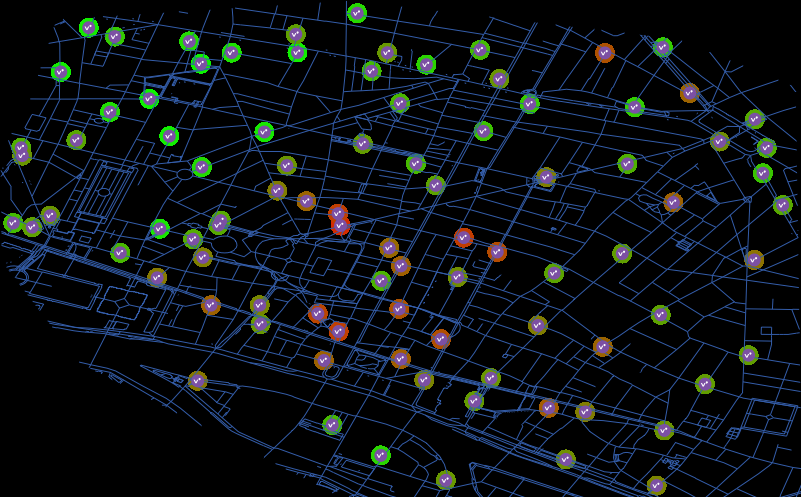
\includegraphics[width=0.6\columnwidth,height=15cm]{figures/lfMidday}
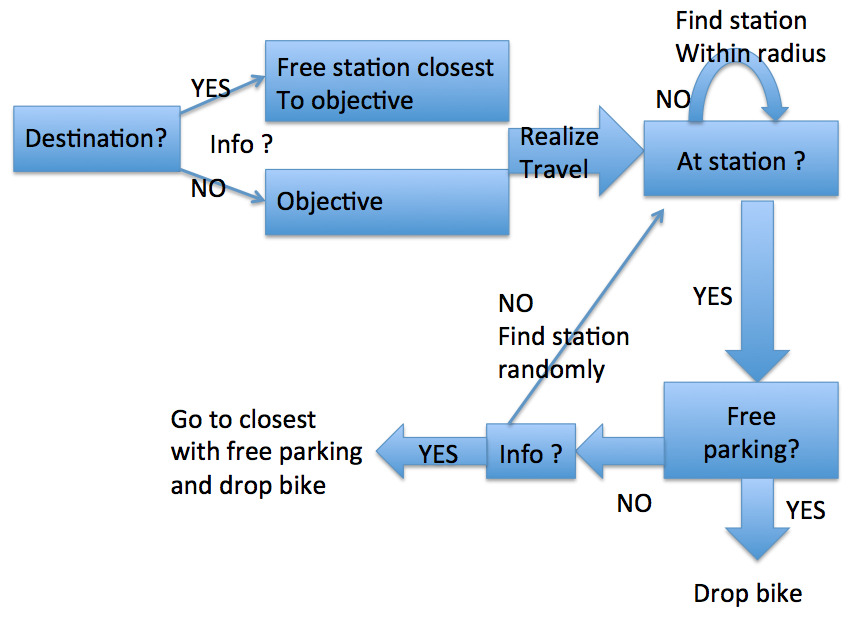
\includegraphics[width=0.4\columnwidth,height=15cm]{figures/flowchart.png}

\textit{\small Left : Example of graphical output of the model. Right : Flowchart of bikers behavior.}


\end{justify}
          \end{column}
          \end{columns}
        \end{block}


        
%%%%%%%%%%%%%%%%%%%%%%%%%%%%%%%%%%%%%%%%%%%%%%%%%%%%%%%%%%%%%%%%%%%%%%%%%%%%%%%%%


        
        \begin{block}{Statistical Analysis of Raw Data for Parametrization}
       \vspace{-2cm}
        \begin{columns}[t]
        \begin{column}{.95\textwidth}
        \begin{justify}
        
        Raw Data on Paris' bike-sharing system dynamics provided publicly by operator, collected each 5s during 6 month. ``Poor'' data : only docking stations status, allows to extract arrivals and departures.
        
        
        
        \begin{columns}[t]
        \begin{column}{.48\textwidth}
        \vspace{0.01cm}
        \hfill
          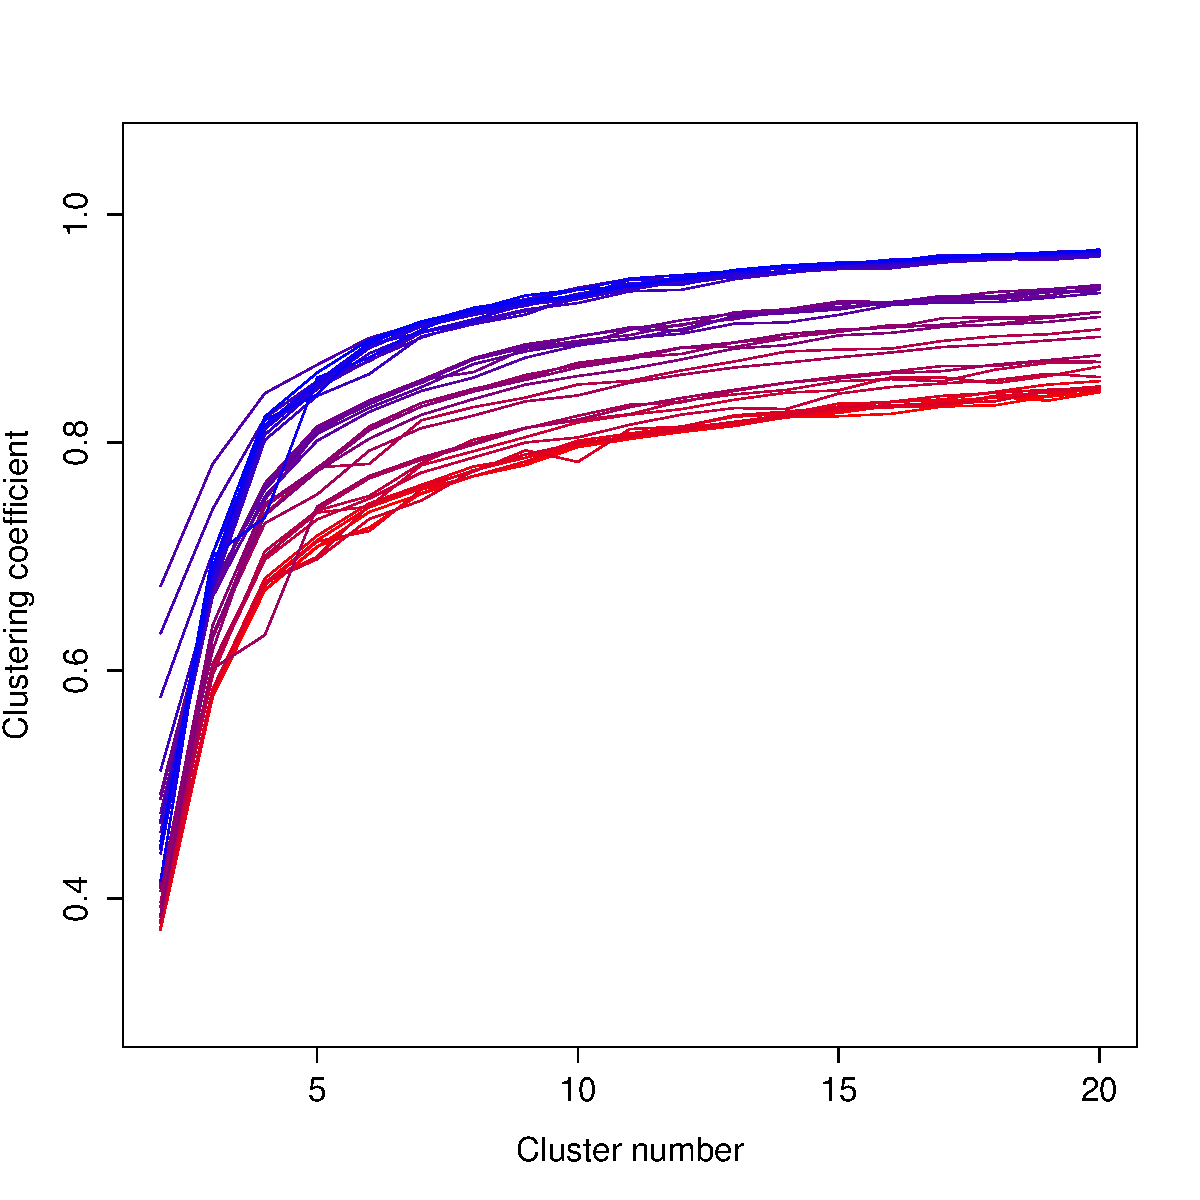
\includegraphics[width=0.5\columnwidth,height=10cm]{figures/clusterNumber}
           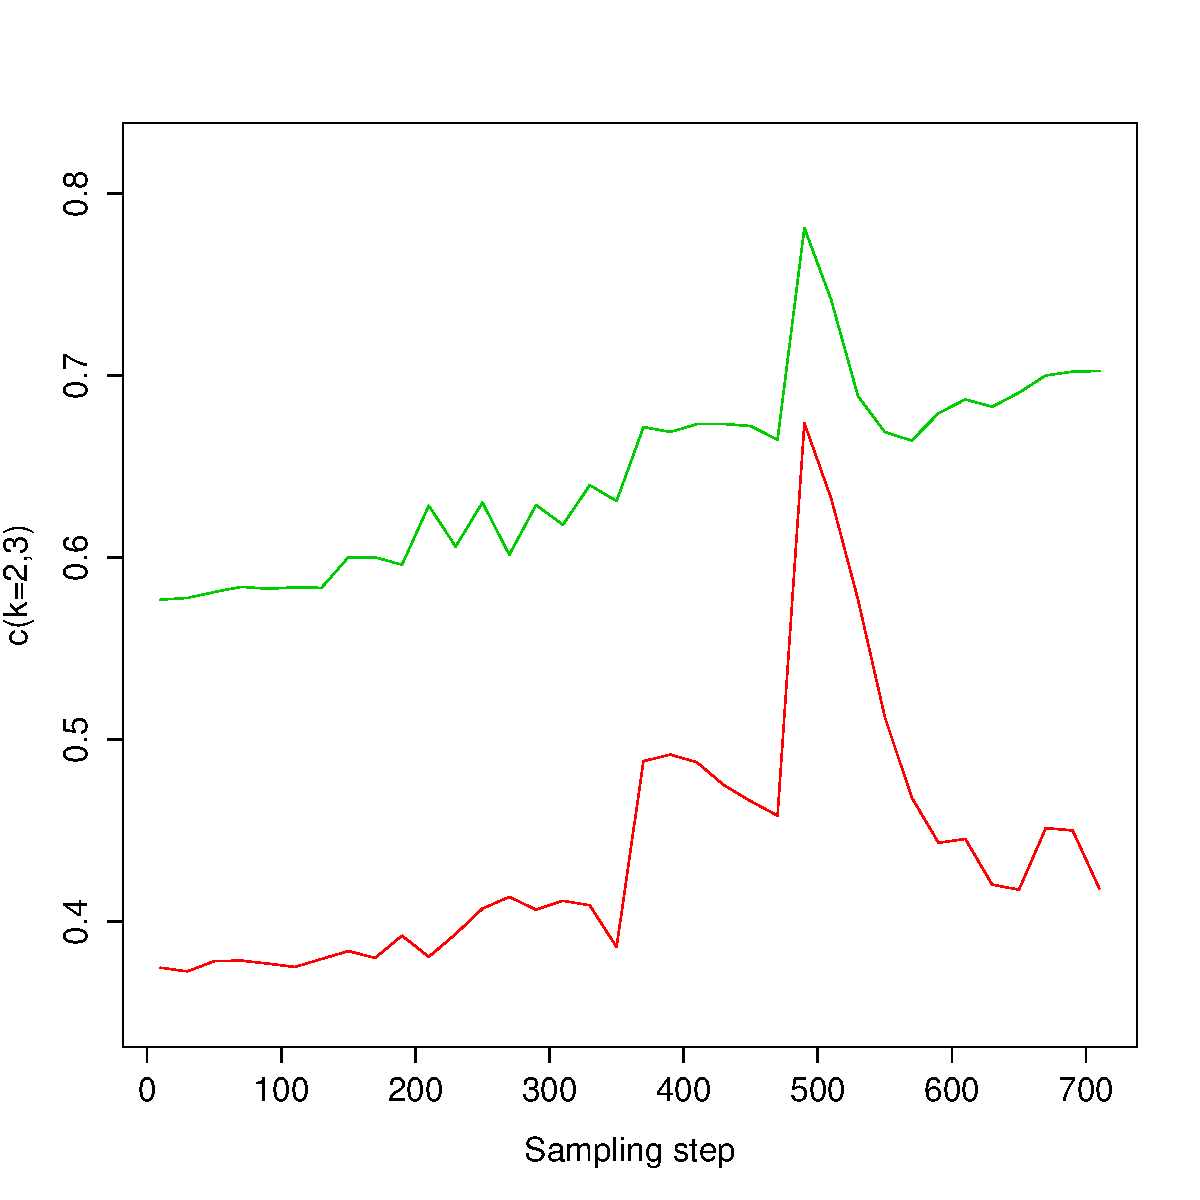
\includegraphics[width=0.5\columnwidth,height=10cm]{figures/infoLoss}
           \hfill\hfill
          \end{column}
          \begin{column}{.48\textwidth}
          \begin{justify}
          %\vspace{-9cm}
          \textit{\small Clustering Analysis of raw data to isolate the patterns of a typical day. Dimension reduction by clustering on stations (Left : role of cluster number) and time-series sampling (Right : effect of sampling step on information).}
          \end{justify}
          \end{column}
          \end{columns}

        
        
        \vspace{0.5cm}
        
        O/D fields are then estimated by a multi-kernel estimation, similarly to Geographically Weighted Regression~\cite{brunsdon2002geographically}, with $(d_{i}(t))$
real arrivals at $(\vec{x}_{i}(t))$,
        
        \[
[D(t)](\vec{x})=\frac{1}{K}\sum_{i}d_{i}(t)\cdot \exp\left(\frac{\left\Vert \vec{x}-\vec{x}_{i}\right\Vert }{2\sigma^{2}}\right)
\]
        

          \end{justify}
          \end{column}
          \end{columns}
        \end{block}
        
        
%%%%%%%%%%%%%%%%%%%%%%%%%%%%%%%%%%%%%%%%%%%%%%%%%%%%%%%%%%%%%%%%%%%%%%%%%%%%%%%%%
 

         
        
      \end{column}
      
%%%%%%%%%%%%%%%%%%%%%%%%%%%%%%%%%%%%%%%%%%%%%%%%%%%%%%%%%%%%%%%%%%%%%%%%%%%%%%%%%
  

      
      \begin{column}{.49\textwidth}

%%%%%%%%%%%%%%%%%%%%%%%%%%%%%%%%%%%%%%%%%%%%%%%%%%%%%%%%%%%%%%%%%%%%%%%%%%%%%%%%%


    \vspace{-0.5cm}
    
%%%%%%%%%%%%%%%%%%%%%%%%%%%%%%%%%%%%%%%%%%%%%%%%%%%%%%%%%%%%%%%%%%%%%%%%%%%%%%%%%
        
        \begin{block}{Validation and Calibration}
       \vspace{-1cm}
       \begin{columns}[t]
        \begin{column}{.95\textwidth}
       
       \vspace{-1cm}
       
       \begin{justify}
       

       Reduced parameter space to be explored contains $p_I$ proportion of user having access to information, $\bar{r}$ mean tolerated walking radius and $\sigma$ kernel size. Grid exploration with repetitions, use of \texttt{OpenMole} software for systematic model exploration~\cite{reuillon2013openmole}.
       
         \end{justify}
    
    \vspace{-1cm}
       
        \begin{columns}[t]
        \begin{column}{.47\textwidth}
                    
          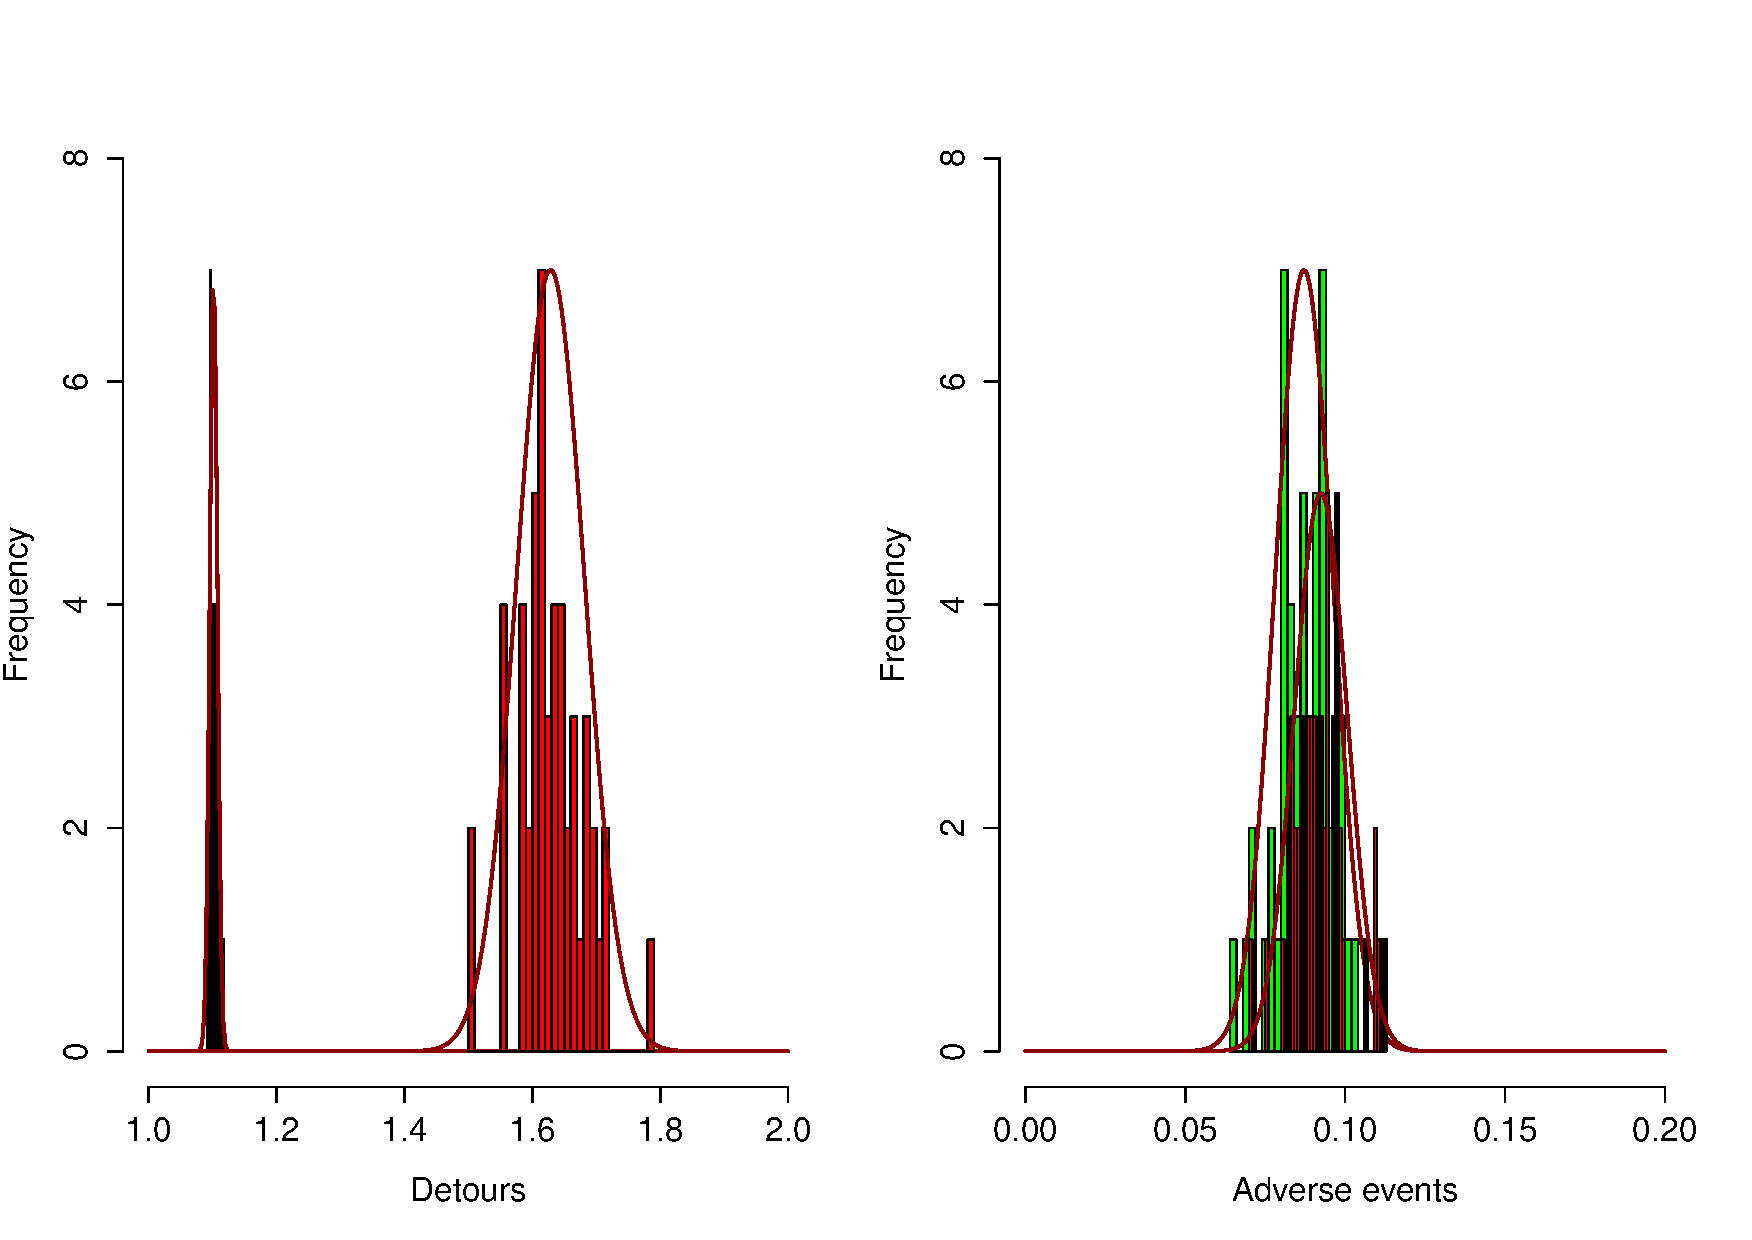
\includegraphics[width=0.9\columnwidth,height=11cm]{figures/histogram}\\
  \begin{justify}
          \textit{\small Internal validation : distributions of indicators for different parameter values.}
 \end{justify}

          \end{column}
          \begin{column}{.47\textwidth}
         
           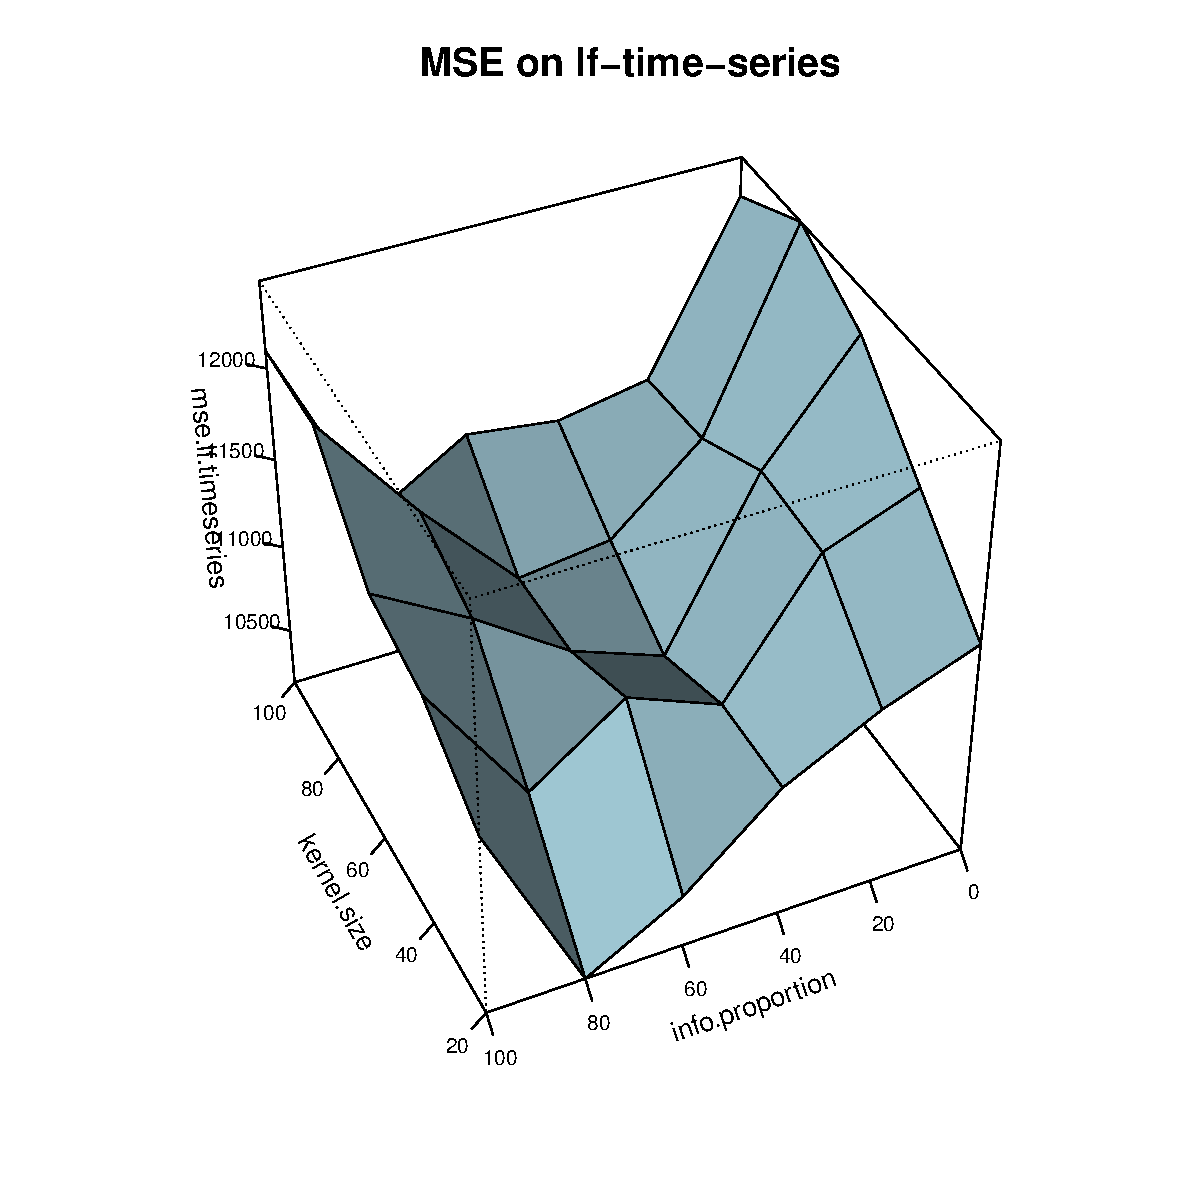
\includegraphics[width=0.9\columnwidth,height=11cm]{figures/calib3d}\\
             \begin{justify}
       \textit{\small Calibration : minimization of MSE on $(p_I,\sigma)$ plane.}
    \end{justify}
    
          \end{column}
          \end{columns}
          \end{column}
          \end{columns}
          
        \end{block}
  

%%%%%%%%%%%%%%%%%%%%%%%%%%%%%%%%%%%%%%%%%%%%%%%%%%%%%%%%%%%%%%%%%%%%%%%%%%%%%%%%%
    
   
%%%%%%%%%%%%%%%%%%%%%%%%%%%%%%%%%%%%%%%%%%%%%%%%%%%%%%%%%%%%%%%%%%%%%%%%%%%%%%%%%



  
      
        \begin{block}{Application : User-based Improvement Strategy}
          \begin{columns}[t]
        \begin{column}{.95\textwidth}
        \begin{justify}
        \vspace{-2cm}
            
          We test the influence of user parameters such as quantity of information or propensity to walk on the performances of the system.
          
          \bigskip
 
\hfill
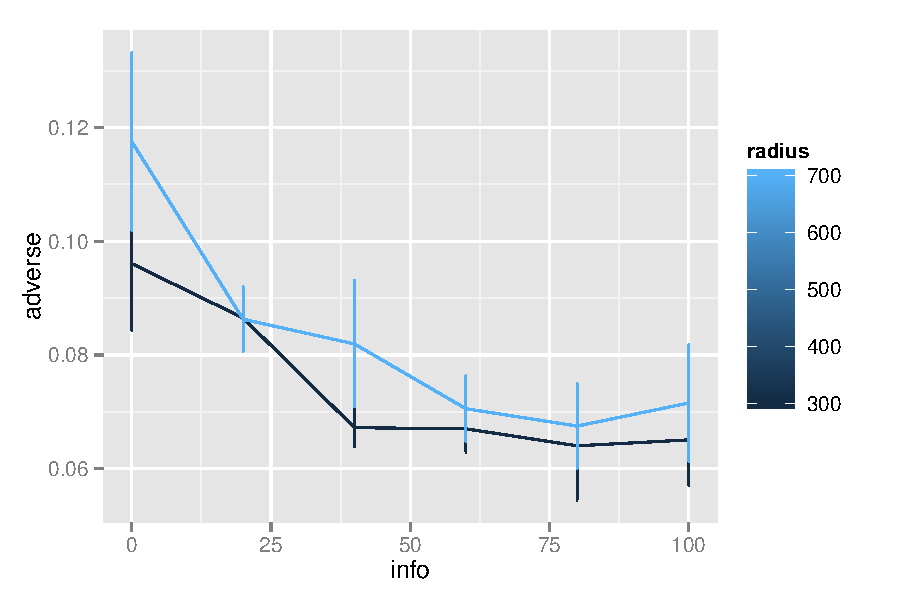
\includegraphics[width=0.45\columnwidth]{figures/adverse}
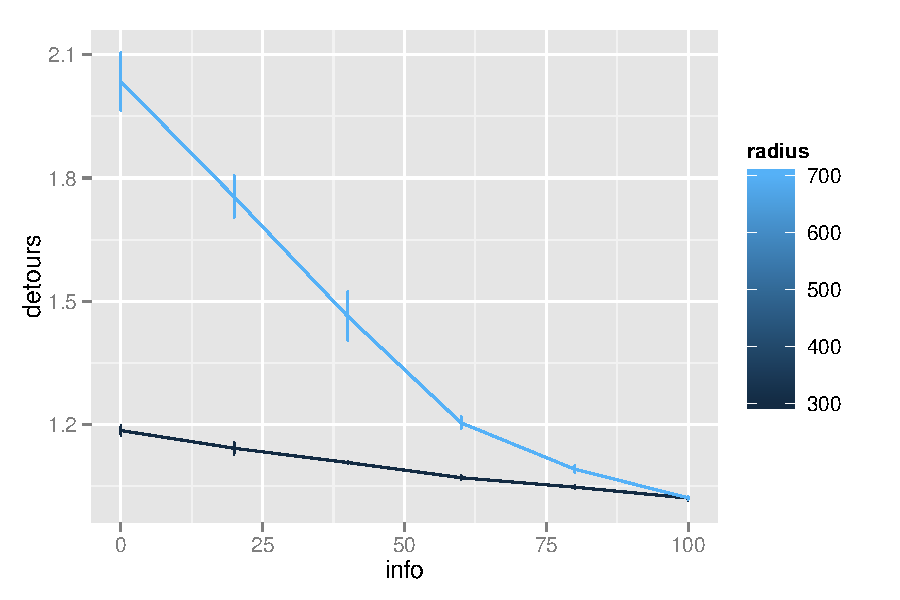
\includegraphics[width=0.45\columnwidth]{figures/detours}
     \hfill
\hfill

\textit{\small Influence of information proportion on adverse events (left) and on quantity of detours (right) for different values of walking radius. We observe a saturation of performance improvement at a low value $p_I\simeq 30\%$.}

\bigskip



          
          
          \end{justify}
          \end{column}
          \end{columns}
        \end{block}

%%%%%%%%%%%%%%%%%%%%%%%%%%%%%%%%%%%%%%%%%%%%%%%%%%%%%%%%%%%%%%%%%%%%%%%%%%%%%%%%%



        \begin{block}{Extension : Discrete Choices Model for User Behavior}
        \vspace{-2cm}
          \begin{columns}[t]
        \begin{column}{.95\textwidth}
        
        \begin{itemize}
       \item  \begin{justify}Flexibility of model allows to test other rules for user behavior. We extend the model with a Discrete Choices module for the choice between waiting ($w$) and moving ($m$) on at a full docking station, where utilities are, with $t_w$ expected waiting time, $d(i)$ expected detour, $\tilde{d}(i)$ expected distance difference to destination, \end{justify}
        
        \vspace{-1cm}
        \[
U_w(i)=\beta_t t_w + \beta_d \tilde{d}(i) \cdot i + \varepsilon_w
 \textrm{ and }
U_m(i)=\beta_t \frac{d(i)}{\bar{v}} + \beta_d \tilde{d}(i) \cdot i + \varepsilon_m
\]



\item\begin{justify}Data from a questionnaire~\cite{bourcet2014vlib} aimed to estimate above DC parameters (among others) but with poorly significant estimates ($N=150$), to obtain their feasible space.
\end{justify}

\item\begin{justify}Extended parameter space can then be explored, calibration allowing to extract better indirect estimates of DC parameters. First results of directed gradient and grid explorations give rather ``chaotic'' MSE surfaces, would need finer grain exploration (computational limit).
\end{justify}



\end{itemize}

        
          \end{column}
          \end{columns}
        \end{block}


%%%%%%%%%%%%%%%%%%%%%%%%%%%%%%%%%%%%%%%%%%%%%%%%%%%%%%%%%%%%%%%%%%%%%%%%%%%%%%%%%


        \begin{block}{Conclusion}
         \begin{columns}[t]
        \begin{column}{.95\textwidth}
         \vspace{-2cm} 
          \begin{justify}
          \begin{itemize}
          \item Simple hybrid model gives interesting thematic results, confirming the potential of ``poor'' datasets.
          \item Methodology of indirectly estimating DC parameters through ABM calibration could be generalized to other types of system.
          \end{itemize}
          \end{justify}
          \end{column}
          \end{columns}
       \end{block}
        
        
%%%%%%%%%%%%%%%%%%%%%%%%%%%%%%%%%%%%%%%%%%%%%%%%%%%%%%%%%%%%%%%%%%%%%%%%%%%%%%%%%        
        
        
        \begin{block}{References}
        
        \fontsize{15}{3}
        \vspace{-2cm}
        
        \begin{multicols}{2}
        \begin{justify}
          \bibliographystyle{apalike}
          \bibliography{biblio/bikesDiscreteChoices,biblio/bibtex,biblio/dynamite}
        
        \end{justify}
          \end{multicols}
        \end{block}
        
        
      \end{column}
    \end{columns}
  \end{frame}
\end{document}





